\documentclass[tikz, dvisvgm, border=5mm]{standalone}
\usetikzlibrary{calc, angles, quotes}

\begin{document}
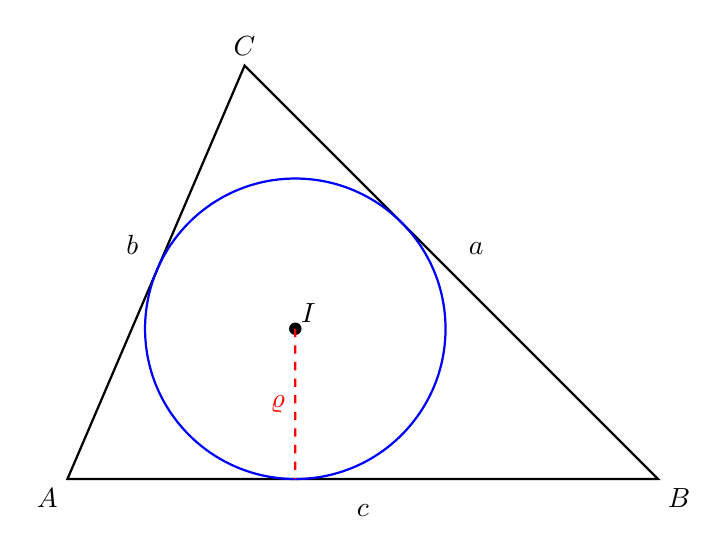
\begin{tikzpicture}[scale=1.5]

    % 1. Definition der Eckpunkte (Allgemeines/schiefwinkliges Dreieck)
    \coordinate (A) at (0,0);
    \coordinate (B) at (5,0);
    \coordinate (C) at (1.5,3.5);

    % Berechneter Inkreismittelpunkt (I) und Radius (r)
    % I liegt exakt bei (1.929, 1.272), der Radius beträgt 1.272
    \coordinate (I) at (1.929, 1.272);

    % 2. Zeichnen des Dreiecks
    \draw[thick] (A) -- (B) -- (C) -- cycle;

    % 3. Ergänzung: Inkreis und Inkreisradius
    % Inkreis zeichnen
    \draw[blue, thick] (I) circle (1.272);
    
    % Inkreismittelpunkt markieren
    \fill[black] (I) circle (1.5pt) node[above right=-0.5mm] {$I$};
    
    % Inkreisradius (Berührungspunkt auf Seite c liegt direkt unter I)
    \draw[red, thick, dashed] (I) -- (1.929,0) node[midway, left] {$\varrho$};

    % 4. Beschriftung der Ecken und Seiten
    % Ecken
    \node[below left] at (A) {$A$};
    \node[below right] at (B) {$B$};
    \node[above] at (C) {$C$};
    
    % Seiten (mittig platziert mit leichtem Versatz nach außen)
    \path (A) -- (B) node[midway, below=2mm] {$c$};
    \path (B) -- (C) node[midway, above right=1mm] {$a$};
    \path (C) -- (A) node[midway, above left=1mm] {$b$};

\end{tikzpicture}
\end{document}